%% Paper C — UCC 2026 (double-blind). BASE = revisão integral da autora
%% (18-19/08/2026, estilo/clareza) + 6 correções objetivas aplicadas por
%% Edit (ref Zhu, triângulo Tab. I, auditoria cross-domain, evidence
%% debt, frase-tese e desfecho pós-hoc no abstract). Números idênticos
%% aos outputs congelados de e10_eaml (spec v3). Linhagem anterior
%% preservada em main_en_ucc_c_v1.tex.
\documentclass[conference]{IEEEtran}
\IEEEoverridecommandlockouts
\usepackage[T1]{fontenc}
\usepackage[utf8]{inputenc}
\usepackage{cite}
\usepackage{amsmath,amssymb}
\usepackage{graphicx}
\graphicspath{{./}{./figures/}{../figures/}}
\usepackage{booktabs,array,multirow}
\usepackage{tikz}
\usetikzlibrary{arrows.meta,positioning,backgrounds}
\usepackage[hidelinks]{hyperref}
\hypersetup{pdfauthor={Anonymous},pdftitle={From Frame to Episode:
Evidence-Preserving Alert Mediation for Selective Inference in
Vehicular Edge Systems},pdfsubject={},pdfkeywords={},
pdfcreator={LaTeX},pdfproducer={pdfTeX}}
\setlength{\textfloatsep}{7pt plus 1pt minus 2pt}
\setlength{\floatsep}{6pt plus 1pt minus 2pt}
\setlength{\intextsep}{7pt plus 1pt minus 2pt}

\newcommand{\osst}{\mathrm{OSS}_t}
\newcommand{\ttaef}{\mathrm{TTA}_{\mathrm{ef}}}

\title{From Frame to Episode: Evidence-Preserving Alert Mediation for Selective Inference in Vehicular Edge Systems}

\author{
\IEEEauthorblockN{Anonymous Authors}
\IEEEauthorblockA{Paper submitted for double-blind review}}

\begin{document}
\maketitle

\begin{abstract}
Vehicular edge nodes often reduce per-frame computation to meet latency
and energy constraints. This strategy, however, can remove information
that the alerting layer still needs to determine whether an alert should
be delivered. When frames are skipped and previous predictions are
reused, the system may no longer know whether the available evidence is
sufficiently current to support an alert.
We present a cognitive edge architecture that separates \emph{when to
compute} from \emph{when to alert} across four decision levels and makes
suppression itself first-class, auditable evidence. A
Suppression Summary produced by the Operational State and Suppression
Layer (OSSL) records information about every skipped frame at constant
cost, without inferring a new risk estimate. An Episodic Alert Mediation
Layer (EAML) is the single origin of driver alerts and requests fresh
computation whenever high episodic risk is supported by
reuse-dominated evidence.
The architecture was evaluated in a controlled synthetic
vehicular-risk environment using separate development seeds and an
internally frozen 20-seed holdout. First, we compared the proposed
architecture with a legacy frame-level trigger and an event-governed
safeguard baseline that does not use suppression evidence. The full
mediation satisfied the complete pre-declared admissibility
specification. Event recall increased by 0.021 (95\% CI
$[0.006,0.037]$) with effective-latency parity, false alerts per trip
decreased by 62\%, and the stale-alert rate decreased from 0.030 to
zero. Removing the Suppression Summary made the design inadmissible and
reintroduced stale alerts (+0.0066, CI $[0.005,0.008]$). Together with
the mechanism-decomposition analysis, this supports mechanism-level
attribution under the evaluated simulation assumptions.
Second, under an oscillating-risk stress regime, the legacy trigger
produced 13.1 alerts per trip, while the event-governed baseline lost
approximately two thirds of its recall. The mediated architecture
retained substantially more coverage than the governed baseline and
maintained zero stale alerts, although no evaluated arm satisfied the
alert budget in this stress regime. Finally, post-hoc analyses separated
the effects of evidence preservation and forced refresh, and showed
that the results are not artifacts of the stale-alert accounting
threshold or of baseline calibration. These results validate the
architectural mechanism under controlled simulation assumptions;
evaluation with naturalistic driving data and embedded hardware remains
future work.
\end{abstract}

\begin{IEEEkeywords}
edge--cloud continuum, edge AI, selective computation, alert governance,
self-adaptive systems, evidence architecture, vehicular safety,
reproducibility
\end{IEEEkeywords}

\section{Introduction}
\label{sec:intro}

Real-time driving-risk detection at the edge must balance three
requirements: low latency, limited resource use, and reliable
communication with the driver~\cite{shi2016edge,liu2019autonomous}.
Selective computation helps satisfy the first two by suppressing
redundant model updates and reusing previous
predictions~\cite{campos2018skiprnn,graves2016act}. Alert delivery,
however, is decided by a separate mechanism. This creates an important
interaction between computation and communication: the alerting layer
may depend on information that selective computation removes. When a
gate skips a frame, the skipped instant often leaves no record beyond a
reused probability. Downstream components may therefore be unable to
distinguish a newly computed risk estimate from one that has been reused
across several frames without re-evaluation.

This observation motivates the design question addressed in this work:
what information must be preserved when computation is skipped so that
alert decisions remain well grounded? We focus on two failure modes.
The first arises when frame-level alert triggers are combined directly
with temporal governance mechanisms such as thresholds, cooldowns, and
re-arming. In this setting, the trigger controls when an alert is
requested, whereas the safeguard controls whether and when it is
actually delivered. As a result, fast threshold crossing does not
necessarily imply timely or appropriate driver notification. The second
failure mode arises when skipped computation leaves no explicit evidence
about the quality of the reused state. The alerting layer can then act
on evidence whose freshness it cannot assess. We refer to alerts issued
from evidence windows dominated by reused computation as
\emph{stale alerts}. Improving the detector alone does not address
either problem because both concern where and how alert decisions are
made.

We address these failure modes with a cognitive edge architecture
organized into four decision levels (Fig.~\ref{fig:arch}). The levels
separate four questions that are often handled by a single
threshold-based pipeline. Level~1, the Multimodal Hybrid Execution Gate
(MHEG), decides whether the detector should execute on the current
frame. Its decision is based on input variation and predictive
uncertainty, and it is limited to computation scheduling. Level~2, the
Operational State and Suppression Layer (OSSL), records what remains
known when computation is skipped. Every frame produces exactly one
evidence object: either a computed state $z_t$ or a Suppression Summary
$\osst$. The skipped computation is therefore explicitly represented
rather than silently discarded. Level~3, the Episodic Alert Mediation
Layer (EAML), decides whether accumulated evidence is sufficient to
deliver an alert. It is the single origin of driver alerts, aggregates
$z_t$ and $\osst$ over an evidence window, computes episodic risk, and
applies an event-governed delivery rule. When high episodic risk is
supported by evidence dominated by reuse, the EAML requests fresh
computation before deciding whether to alert. Level~4, the cloud,
governs slower configuration changes for future operation. It may
promote new policy parameters but does not bypass local mediation or
trigger driver alerts directly.

The paper makes three contributions. First, we introduce an
\emph{evidence-preserving architecture} for edge alert governance with
explicit invariants at each decision level. Its central requirement is
that skipped computation must leave auditable evidence, at constant
per-frame cost, for the component responsible for communication.
Second, we define the \emph{stale-alert rate} (SAR), an operational
metric that measures the fraction of delivered alerts whose evidence
window is dominated by reused computation. Third, we provide a
confirmatory evaluation of the architecture using a protocol frozen
before a 20-seed holdout. The evaluation includes a documented amendment
trail in which two earlier specifications produced empty admissible
sets, an ablation designed to test the role of suppression evidence, and
an oscillating-risk stress analysis that examines behavior outside the
nominal evaluation regime.

The evaluation is organized around three research questions that move
from overall effect to mechanism and then to behavior under stress.
\emph{RQ1}: Does episodic mediation improve alert quality over an
event-governed safeguard baseline without sacrificing recall or
effective latency, while remaining within a declared alert budget?
\emph{RQ2}: Does suppression evidence contribute to that improvement, or can the mediation succeed without it?
\emph{RQ3}: How do the competing designs behave under an
oscillating-risk regime that stresses the interaction between selective
computation and alert delivery?

\section{Related Work}
\label{sec:related}

The design space addressed in this work lies at the intersection of four
research areas: selective computation, streaming risk detection, runtime
assurance, and information freshness. Each contributes part of the
solution, but none directly addresses how alerting should reason about
evidence that was not freshly computed.

\textbf{Selective and adaptive computation.} Skip
RNN~\cite{campos2018skiprnn}, adaptive computation
time~\cite{graves2016act}, adaptive frame
selection~\cite{wu2019adaframe}, and coarse-to-fine
inference~\cite{wu2019liteeval} reduce the cost of recurrent or video
models by suppressing unnecessary updates or selecting more informative
inputs. Their primary objective is computational efficiency while
preserving task performance. In these approaches, however, a skipped
instant is typically represented only through the reuse of an earlier
state or prediction. The skipped computation itself does not produce an
explicit evidence object that records what was omitted, how long the
reused state has persisted, or how the input evolved during that period.
MOSAIC~\cite{gokarn2023mosaic} is a closer point of comparison because it
tracks prediction age and reuse across concurrent video streams for
criticality-aware scheduling. That information is used to support
resource allocation, rather than downstream alert decisions. In our
architecture, selective computation remains a scheduling mechanism at
the first level, while the downstream consequences of suppression are
represented explicitly for later decision making.

\textbf{Streaming risk detection and online action detection.} Causal
recurrent methods for driver monitoring~\cite{sajid2021,fresta2025} and
online action detection~\cite{xu2021oad} focus on producing reliable
predictions under strict temporal causality, usually evaluated with
detection-oriented aggregate metrics. A separate body of work on
collision-warning systems shows that the usefulness of a warning also
depends on when it is delivered and on how often false or redundant
alerts occur~\cite{abe2006timing,bliss2003alarm}. These results motivate
evaluating the \emph{delivered alert}, rather than the frame-level
detection score alone. What is generally not modeled in this literature
is the interaction between alert delivery and selective computation,
especially when an alert decision depends on predictions that may have
been reused across skipped frames.

\textbf{Runtime assurance and self-adaptive systems.} Runtime assurance
architectures mediate proposed actions before
execution~\cite{seto1998simplex,alshiekh2018shield}, while autonomic and
self-adaptive systems organize adaptation through feedback loops such as
MAPE-K over shared knowledge~\cite{kephart2003,weyns2020}. These
perspectives motivate two boundaries in our architecture. Decisions that
affect the driver are mediated locally at the edge, whereas slower
configuration changes are handled separately through governed policy
promotion in the cloud. The remaining question is what information the
local alerting layer can rely on when selective computation means that
many frames were never freshly evaluated. Our work addresses this
within-edge evidence problem rather than proposing a new runtime
assurance or self-adaptation mechanism.

\textbf{Information freshness and age-aware systems.} Age-of-information
(AoI) research studies the timeliness of updates and its effect on
decisions in networked and edge systems~\cite{yates2021aoi}. Related work has examined
how stale observed features affect real-time inference
accuracy~\cite{shisher2022freshness} and how peak-age objectives can guide
scheduling or forced updates~\cite{zhu2026paoi}. These approaches reason
primarily about the age of data or updates. Our concern is different: an
alert may be delivered at the current time while still being supported
mostly by reused inference evidence. The stale-alert rate (SAR) therefore
measures the composition of the evidence window that supports a delivered
alert, rather than the transport age of the alert or the age of the latest
update. Freshness-aware sensing provides a related mechanism by suppressing
or requesting sensor updates according to age or uncertainty
~\cite{bui2024timely}. In that setting, freshness control acts on sensing
and transmission. Here, freshness is evaluated at the alert-decision
layer, which may request fresh inference before a driver notification is
delivered.

Taken together, these lines provide the individual mechanisms needed for
selective execution, temporal detection, safeguarded delivery, and
freshness-aware control. In the literature reviewed here, however,
including a structured cross-domain audit of the four lines above, we
did not find an evaluated architecture that combines a per-frame evidence
contract for suppressed computation with episodic alert mediation under an
explicit alert budget. The novelty is not a new gating rule, age
metric, safeguard, or forced-update mechanism in isolation. It is a
per-frame evidence contract that makes skipped computation explicitly
observable to downstream decision layers, combined with two
architectural invariants: every frame produces exactly one evidence
object, and every driver alert originates from evidence-aware episodic
mediation. Fresh inference may be requested when the evidence
supporting a candidate alert is dominated by reused computation. Table~\ref{tab:position} summarizes this
positioning.

\begin{table}[!t]
\caption{Positioning of representative mechanisms.}
\label{tab:position}
\centering
\footnotesize
\setlength{\tabcolsep}{2.8pt}
\renewcommand{\arraystretch}{1.10}
\begin{tabular}{@{}lccccc@{}}
\toprule
Mechanism & SE & EA & DS & AB & SA\\
\midrule
Skip RNN / ACT~\cite{campos2018skiprnn,graves2016act}
& -- & -- & -- & -- & --\\
AdaFrame / LiteEval~\cite{wu2019adaframe,wu2019liteeval}
& -- & -- & -- & -- & --\\
MOSAIC~\cite{gokarn2023mosaic}
& $\triangle$ & -- & -- & -- & --\\
Runtime assurance~\cite{seto1998simplex,alshiekh2018shield}
& -- & -- & \checkmark & -- & --\\
AoI / freshness~\cite{yates2021aoi,shisher2022freshness,zhu2026paoi}
& -- & -- & -- & -- & $\triangle$\\
Freshness-aware sensing~\cite{bui2024timely}
& -- & -- & -- & $\triangle$ & $\triangle$\\
\addlinespace[1.5pt]
Event-governed safeguard
& -- & event & \checkmark & \checkmark & --\\
\addlinespace[1.5pt]
\textbf{This work (OSSL+EAML)}
& \textbf{\checkmark} & \textbf{\checkmark} &
\textbf{\checkmark} & \textbf{\checkmark} &
\textbf{\checkmark}\\
\bottomrule
\end{tabular}

\vspace{2pt}
\parbox{\columnwidth}{\footnotesize
SE: suppression evidence; EA: episodic alerting;
DS: delivery safeguard; AB: alert budget; SA: staleness audit.
$\triangle$ denotes a related notion without an explicit
suppression-evidence contract for delivered-alert mediation.
The event-governed safeguard is the frozen A1 baseline, not prior work.}
\end{table}

\section{Architecture: Four Decision Levels}
\label{sec:arch}

The gaps identified above motivate separating four decisions that are
often handled by a single threshold-driven pipeline: when to compute,
what evidence to retain when computation is skipped, when to deliver an
alert, and when to change the operating configuration. We consider a
strictly causal stream of frames $x_t\in\mathbb{R}^{D}$ containing
kinematic, behavioral, and contextual attributes. When executed, a
recurrent detector~\cite{hochreiter1997} produces a risk probability
$p_t$. Consecutive frames are grouped into episodes of length $T$, and
critical episodes contain a risk onset instant $t_{\mathrm{onset}}$.

Figure~\ref{fig:arch} shows how these decisions are separated across
the four levels.

\begin{figure}[!t]
\centering
\resizebox{0.92\columnwidth}{!}{%
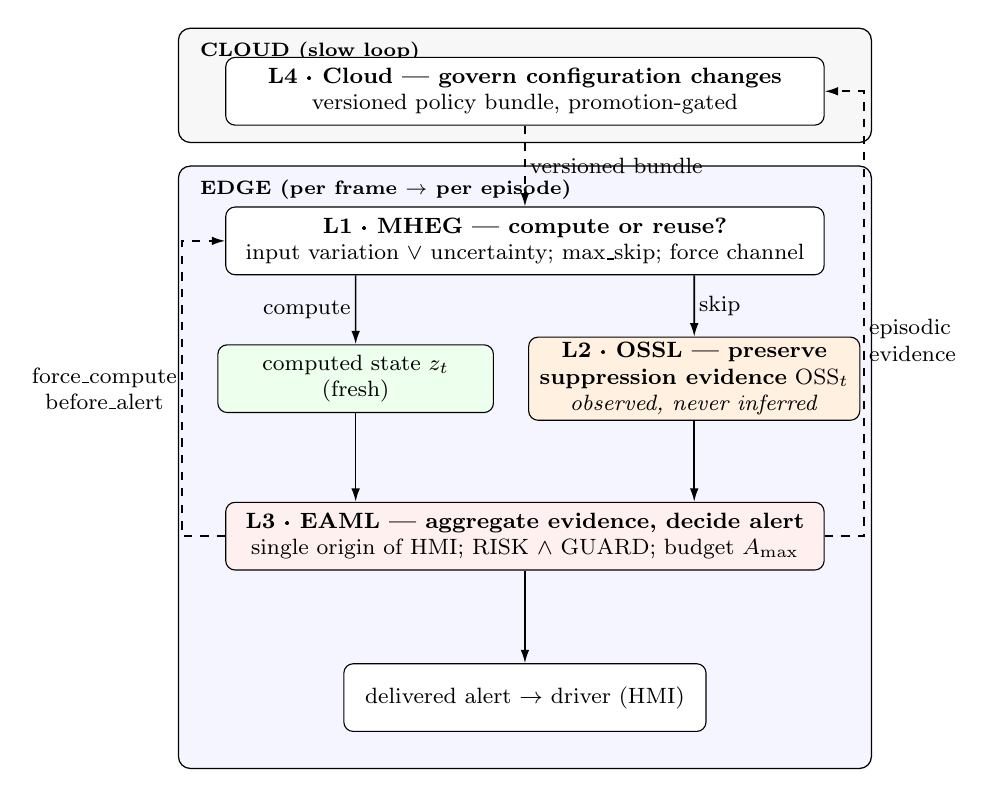
\begin{tikzpicture}[
  font=\footnotesize,
  lvl/.style={draw,rounded corners=1.2mm,fill=white,align=center,
              minimum height=8.6mm,inner xsep=4pt,inner ysep=2pt},
  arr/.style={-{Latex[length=1.7mm,width=1.1mm]},line width=.6pt},
  dasharr/.style={arr,dashed}
]
\draw[rounded corners=1.5mm,fill=black!3,line width=.45pt]
  (-0.2,7.6) rectangle (8.6,9.05);
\node[anchor=north west,font=\scriptsize\bfseries] at (-0.05,9.0)
  {CLOUD (slow loop)};
\node[lvl,minimum width=7.6cm] (cloud) at (4.2,8.25)
  {\textbf{L4 · Cloud — govern configuration changes}\\
   versioned policy bundle, promotion-gated};

\draw[rounded corners=1.5mm,fill=blue!4,line width=.45pt]
  (-0.2,-0.35) rectangle (8.6,7.3);
\node[anchor=north west,font=\scriptsize\bfseries] at (-0.05,7.25)
  {EDGE (per frame $\to$ per episode)};

\node[lvl,minimum width=7.6cm] (mheg) at (4.2,6.35)
  {\textbf{L1 · MHEG — compute or reuse?}\\
   input variation $\vee$ uncertainty; max\_skip; force channel};

\node[lvl,minimum width=3.5cm,fill=green!7] (zt) at (2.05,4.6)
  {computed state $z_t$\\(fresh)};
\node[lvl,minimum width=3.9cm,fill=orange!12] (oss) at (6.35,4.6)
  {\textbf{L2 · OSSL — preserve}\\\textbf{suppression evidence}
   $\osst$\\\emph{observed, never inferred}};

\node[lvl,minimum width=7.6cm,fill=red!6] (eaml) at (4.2,2.6)
  {\textbf{L3 · EAML — aggregate evidence, decide alert}\\
   single origin of HMI; RISK $\wedge$ GUARD; budget $A_{\max}$};

\node[lvl,minimum width=4.6cm] (hmi) at (4.2,0.55)
  {delivered alert $\to$ driver (HMI)};

\draw[arr] (mheg.south) ++(-2.15,0) -- node[left,inner sep=1.5pt]
  {compute} (zt.north);
\draw[arr] (mheg.south) ++(2.15,0) -- node[right,inner sep=1.5pt]
  {skip} (oss.north);
\draw[arr] (zt.south) -- (zt.south |- eaml.north);
\draw[arr] (oss.south) -- (oss.south |- eaml.north);
\draw[arr] (eaml.south) -- (hmi.north);
\draw[dasharr] (eaml.west) -- ++(-0.55,0) |-
  node[pos=0.25,left,align=center,inner sep=1.5pt]
  {force\_compute\\before\_alert} (mheg.west);
\draw[dasharr] (cloud.south) -- node[right,inner sep=1.5pt]
  {versioned bundle} (mheg.north);
\draw[dasharr] (eaml.east) -- ++(0.5,0) |-
  node[pos=0.22,right,inner sep=1.5pt,align=left]
  {episodic\\evidence} (cloud.east);
\end{tikzpicture}%
}
\caption{Four decision levels. Every frame yields exactly one evidence
object ($z_t$ or $\osst$). The EAML is the only path to the driver's
human--machine interface (HMI), and the cloud changes parameters only
through governed promotion.}
\label{fig:arch}
\end{figure}

\subsection{Level 1 (MHEG): when to compute}

The MHEG is responsible only for computation scheduling. Its question is
whether the current frame contains enough new information to justify
running the detector. The detector executes when the input variation
satisfies $|\Delta x_t|\geq\tau_\Delta$ over a kinematic subset or when
the previous prediction is sufficiently uncertain,
$H(p_{t-1})\geq\tau_H$. A hard limit, max\_skip, bounds the number of
consecutive suppressed frames. The MHEG also exposes a \emph{force
channel} through which higher levels can request an additional detector
execution when fresh evidence is needed.

These decisions are binary: execute the detector or reuse the most recent
computed state. The MHEG remains external to the detector and does not
participate in alert delivery. In the evaluated configuration,
$\tau_\Delta{=}0.005$, $\tau_H{=}0.6$, and max\_skip${=}8$, which
suppresses approximately 68\% of frames.

\subsection{Level 2 (OSSL): suppression as first-class evidence}

Selective computation creates an information gap whenever the detector is
not executed. The Operational State and Suppression Layer (OSSL) makes
that gap explicit through a per-frame evidence contract. Every frame
produces exactly one evidence object: either a freshly computed state
$z_t$, containing $p_t$ and its uncertainty, or a Suppression Summary
$\osst$.

The Suppression Summary does not estimate a new risk probability. Its
purpose is to describe the skipped computation well enough for downstream
components to assess the quality of the reused state. It therefore stores,
in constant space, the source of the reused state and its age, accumulated
and maximum input variation, carried entropy, a confidence-decay
estimate, a low-cost risk proxy, the margins to the two gate thresholds,
the current suppression-run length, and a derived quality tag in
$\{$safe, watch, unsafe$\}$.

Three invariants define the OSSL. (I1) $\osst$ never creates a new risk
probability; suppressed computation is observed and summarized rather
than inferred. (I2) Each summary requires $O(1)$ work and storage per
frame. (I3) Every frame contributes an evidence object, so the evidence
stream contains no gaps. Together, these invariants make suppression
explicit and auditable for downstream mediation and analysis.
Table~\ref{tab:oss} lists the complete Suppression Summary.

\begin{table}[!t]
\caption{The Suppression Summary $\osst$ (per suppressed frame, $O(1)$).}
\label{tab:oss}
\centering\scriptsize
\setlength{\tabcolsep}{4pt}
\begin{tabular}{@{}lp{5.3cm}@{}}
\toprule
Field & Meaning\\
\midrule
reused\_from, elapsed & index and age of the last computed state\\
$\Delta x$, $\max\Delta$ & accumulated and maximum input variation
  since that state\\
entropy\_carried & uncertainty of the reused prediction\\
confidence\_decay & age- and variation-based decay estimate\\
cheap\_risk\_proxy & low-cost kinematic risk indicator\\
trigger\_margins & distances to $\tau_\Delta$ and $\tau_H$ at skip time\\
suppression\_count & length of the current suppression run\\
quality & derived tag in \{safe, watch, unsafe\}\\
\bottomrule
\end{tabular}
\end{table}

\subsection{Level 3 (EAML): when to alert}

The Episodic Alert Mediation Layer (EAML) is the only component allowed
to deliver driver alerts. A high frame-level detector score is therefore
treated as evidence for an alert decision rather than as an alert by
itself. The EAML processes the evidence in a fixed sequence. It first
aggregates the current evidence window, then estimates episodic risk,
applies persistence and escalation logic, evaluates the event-governed
guard, checks evidence freshness, and only then decides whether an alert
should be delivered.

For a sliding window $W$ of evidence objects, episodic risk is

\[
R_E = 0.7\cdot\overline{\text{top-}k}
      + 0.3\cdot\text{peak},
\]

where $\overline{\text{top-}k}$ is the mean of the $k$ highest risk
values in the window and \textit{peak} is the maximum. Delivery requires
both a RISK condition and a GUARD condition. RISK is satisfied by
persistence of $m$ frames above $\theta_{\mathrm{ep}}$, by a peak
condition, or by escalation. GUARD is implemented by the
event-governed safeguard (EGS). An event opens at
$\theta_{\mathrm{on}}$, closes below $\theta_{\mathrm{off}}$, and can
generate another alert only after escalation or lack of driver response,
subject to a minimum gap. The per-trip limit $A_{\max}$ bounds the total
number of delivered alerts.

Three invariants govern this level. (E1) No driver alert is generated
outside the EAML. (E2) A single high-risk frame cannot satisfy the RISK
condition on its own. (E3) If episodic risk is high while more than
60\% of the evidence window is reused and the latest detector execution
is sufficiently old, the EAML issues
\emph{force\_compute\_before\_alert}. The MHEG then performs the requested
computation, after which the EAML re-evaluates the alert decision using
the refreshed evidence. This prevents the system from delivering an alert
solely on the basis of a reuse-dominated evidence window.

\subsection{Level 4 (cloud): adaptation by promotion only}

Level~4 handles slower system adaptation. The parameters
$\tau_\Delta$, $\tau_H$, $W$, $m$, $\theta_{\mathrm{ep}}$, the guard
settings, and $A_{\max}$ are stored in a versioned policy bundle.

The cloud may propose a new bundle, but that bundle reaches the edge only
through a governed promotion decision based on pre-declared criteria over
delivered outcomes. The cloud does not generate driver alerts and does not
override the EAML. Level~4 defines an architectural boundary rather
than an evaluated component. Cloud-side policy promotion is neither
implemented nor experimentally evaluated in this study; it is included
to specify that remote configuration changes cannot bypass local alert
mediation.

\subsection{Threshold provenance and freezing}

The thresholds used by the architecture serve different purposes and
were not all established in the same way. Parameters that control the
mediated alerting policy were selected using development data only and
were frozen before the confirmatory holdout. In particular, the EAML
configuration ($W$, $m$, $\theta_{\mathrm{ep}}$, the guard thresholds,
and $A_{\max}$) was selected from the development search described in
Sec.~\ref{sec:protocol} and then held fixed for confirmatory evaluation.

The MHEG parameters $\tau_\Delta$, $\tau_H$, and max\_skip define the
selective-computation regime used throughout the study. They were fixed
during development to establish the evaluated suppression operating point
and were not tuned using holdout outcomes.

The reuse threshold of $0.60$ serves a different role. It defines a
reuse-dominated evidence window as one in which a strict majority of the
evidence has been reused. The threshold was fixed during development and
was not selected using holdout results. Its sensitivity is examined
post-hoc at $0.50$, $0.60$, and $0.70$.

These architectural thresholds are distinct from the admissibility
criteria of Sec.~\ref{sec:protocol}, which are declared engineering
criteria rather than universal human-factors constants. No
architectural or evaluation threshold was re-optimized using the
confirmatory holdout.

\subsection{Operational metrics}

The evaluation measures five operational properties of the alerting
system: coverage, timeliness, false-alert burden, evidence freshness, and
total alert load.

\emph{Event recall} is the fraction of critical episodes for which at
least one alert is delivered after the risk onset. \emph{Effective
time-to-alert} combines detection delay and missed-event penalty:

\begin{equation}
\ttaef=(t_{\mathrm{alert}}-t_{\mathrm{onset}})\cdot\Delta t
 \;+\;\mathbf{1}[\mathrm{miss}]\cdot T_{\max},
\label{eq:ttaef}
\end{equation}

where $T_{\max}{=}10$\,s. A critical episode that receives no alert is
therefore assigned the maximum delay. The \emph{false-alarm rate}
(FAR) counts alerts delivered during non-critical episodes per trip. The total number of
\emph{alerts/trip} is evaluated against the declared budget
$B{=}2.5$.

Evidence freshness is measured by the \emph{stale-alert rate} (SAR).
For the set $\mathcal{A}$ of delivered alerts,

\begin{equation}
\mathrm{SAR}=\frac{1}{|\mathcal{A}|}\sum_{a\in\mathcal{A}}
 \mathbf{1}\!\left[\rho_W(a) > 0.60\right],
\label{eq:sar}
\end{equation}

where $\rho_W(a)$ is the fraction of reused evidence in the decision
window when alert $a$ is delivered; the provenance of the $0.60$
threshold is described above.

Lower SAR indicates that fewer delivered alerts depend on
reuse-dominated evidence. For example, SAR${=}0.03$ means that 3\% of
delivered alerts were issued from windows classified as stale, whereas
SAR${=}0$ means that no delivered alert met this criterion. SAR should not
be interpreted as the age of the alert itself. It measures how much of the
evidence supporting the alert was reused rather than freshly computed.

Redundant alerts per trip, defined as repeated alerts within an event that
has already been notified, are reported as an additional quality measure.
Accordingly, higher event recall is preferred, while lower
$\ttaef$, FAR, SAR, and redundant-alert counts are better.
Alerts per trip is treated differently: it is an operational cost that
must remain within the declared budget.

\section{Frozen Holdout Protocol}
\label{sec:protocol}

The metrics defined above determine the acceptance logic of the
experiment. A candidate is considered useful only if it preserves
coverage and responsiveness, remains within the declared alert budget,
does not worsen false-alert burden, and improves at least one alert-quality
dimension. These requirements were encoded in an internally frozen
holdout protocol finalized before any inspection of the holdout. The
protocol was not externally preregistered.

All experimental arms use the same episode generator, observation
model, MHEG configuration, and pre-drawn exogenous realizations,
verified by assertion; the arms differ only in the alert-decision
layer.

\subsection{Experimental arms}

Each arm addresses a different experimental question. A0 represents a
conventional unbudgeted frame-level trigger. A1 adds event-governed
delivery but does not use suppression evidence. A2 instantiates the
complete architecture described in Section~\ref{sec:arch}. A3 removes
the suppression-evidence mechanism from A2 and is used as the primary
ablation. A4 is a post-hoc decomposition arm that retains suppression
evidence but disables forced refresh.

\textbf{A0 - Legacy}
A frame-level trigger fires when $p_t\geq\theta$, with cooldown 3 and
hysteresis 0.05. It has no alert budget and serves as the descriptive
as-is reference.

\textbf{A1 - EGS}
The event-governed safeguard baseline uses
$\theta_{\mathrm{on}}{=}0.55$, $\theta_{\mathrm{off}}{=}0.52$, gap 2,
and $A_{\max}{=}3$. Its configuration predates this study and was kept
frozen rather than re-optimized for the confirmatory experiment. A1
governs alert delivery at the event level, but it is not guaranteed to
satisfy the alert budget adopted in this study. Because A1 predates the
current experiment and was not optimized for its alert budget,
conclusions from the primary A2--A1 comparison are interpreted jointly
with the re-optimized safeguard analysis reported in
Section~\ref{sec:mechanism}.

\textbf{A2 - EAML}
The complete mediated architecture described in
Section~\ref{sec:arch}.

\textbf{A3 - EAML$-$OSSL}
This ablation is identical to A2 except that suppressed frames enter the
evidence window without $\osst$. The previous probability is carried
forward without the associated quality or decay information, and the
force channel is disabled.

\textit{A4 -- EAML with OSSL and no forced refresh.}
This post-hoc mechanism-decomposition arm retains the Suppression
Summary but disables the forced-refresh channel. It is not included in
the pre-declared admissibility analysis and is used only to separate
the effects of evidence preservation and freshness restoration.

\subsection{Scenarios and experimental design}

Each episode contains $T{=}96$ frames (${\approx}10$\,s) and
$D{=}31$ attributes. Episodes are generated from behavioral recipes
covering normal (N01--N03), attention (A01--A03), borderline
(L01--L03), abrupt-critical (C01--C04), and progressive-critical
(C05--C10) patterns. The borderline recipes are the primary source of
false alerts. Feature and risk calibration are derived from
naturalistic-driving statistics~\cite{dingus2016shrp2}.

Twelve synthetic driver personas represent distinct behavioral
profiles, each defined by three modifiers: risk exposure, responsiveness
to alerts, and fatigue, which degrades that response. The personas
exist so that the results do not depend on a single behavioral profile.
Each persona drives 20 trips, and each trip is a sequence of 12
episodes, so one seed contains $12\times20\times12=2{,}880$ episodes;
a seed is one complete repetition of the simulated world with different
pre-drawn random realizations. The fixed recipe mix of
50/15/15/10/10\% determines how these 2{,}880 episodes are distributed
over the five families: 1{,}440 normal, 432 attention, 432 borderline,
288 abrupt-critical, and 288 progressive-critical episodes.

This design fixes the evaluation denominators. Each seed contains 576
critical episodes (the abrupt and progressive families, 20\% of the
mix), over which event recall is computed, and 2{,}304 non-critical
episodes, over which false alerts are counted; the 20 holdout seeds
therefore comprise 57{,}600 episodes. The trip is the operational unit:
alert load and FAR are reported per trip, and the total load is
compared with the declared budget $B$. Because the recipe mix is fixed
and all exogenous realizations are pre-drawn and shared, every arm
faces exactly the same episode sequence, so outcome differences are
attributable to the alert-decision layer alone.

The observation model is declared rather than learned. Observed risk is

\[
p_{\mathrm{obs}}(t)=
\mathrm{clip}\!\left(
y(t)+\varepsilon_t\cdot0.10\cdot(1.2-\omega)
\right),
\]

where $y(t)$ is the latent risk defined by the recipe,
$\varepsilon_t\!\sim\!\mathcal{N}(0,1)$ is pre-drawn, and $\omega$ is
the persona-specific observability parameter. The entropy supplied to the
MHEG is computed from the most recent detector prediction. Driver response
follows

\[
q=\mathrm{clip}(\mathrm{resp}-0.4\cdot\mathrm{fatigue},0.05,1),
\]

with the same pre-sampled uniform realizations used for every arm.

Statistical attribution is performed at the
persona$\times$seed cluster level. Paired differences are aggregated per
cluster before inference~\cite{law2015}. All intervals were computed
from the 240 paired persona$\times$seed cluster differences using a
normal approximation, the mean difference $\pm\,1.96$ standard errors
for the two-sided 95\% intervals, with the standard error estimated
from the sample variance of the cluster differences. The
persona$\times$seed cluster, rather than the individual episode or
alert, was the unit of inference. Stochastic episode realizations
(recipe selection, observation noise, and driver-response draws) were
distinct for every persona$\times$seed combination and never reused
across combinations; common random numbers were shared only across
experimental arms within the same combination. U90 denotes the upper endpoint of the
corresponding two-sided 90\% interval
($\text{mean}+1.645\,\text{SE}$), used by the admissibility gates as a
conservative one-sided upper bound.

Development used seeds 201--205 to select the EAML operating
configuration from a grid of 162 candidates over window length,
persistence, episodic threshold, and guard parameters. The frozen
configuration is $W{=}8$, $m{=}3$, $\theta_{\mathrm{ep}}{=}0.70$ with
guard parameters $\theta_{\mathrm{on}}{=}0.65$,
$\theta_{\mathrm{off}}{=}0.62$, gap 2, and $A_{\max}{=}4$.
The 20 holdout seeds, corresponding to 240 persona$\times$seed clusters,
were generated once, remained uninspected during development, and were
executed exactly once after the configuration was frozen.

\subsection{Admissibility gates and amendment trail}

The admissibility specification translates these operational objectives
into explicit decision criteria. Relative to the governed baseline A1, a candidate is admissible only if
all of the following conditions hold simultaneously:

\begin{align*}
&\mathrm{G1}\;\; \mathrm{U90}(\Delta\ttaef) < +1.0\,\mathrm{s}
 \quad\text{(non-inferior latency)}\\
&\mathrm{G2}\;\; \Delta\mathrm{Recall} \geq -0.02
 \quad\text{(non-inferior coverage, per regime)}\\
&\mathrm{G3}\;\; \mathrm{Alerts/trip} \leq 2.5
 \quad\text{(absolute budget)}\\
&\mathrm{G4}\;\; \mathrm{U90}(\Delta\mathrm{FAR}) \leq 0
 \quad\text{(no false-alert regression)}\\
&\mathrm{G5}\;\; \text{superiority in}\;{\geq}1\;\text{of}\;
 \{\mathrm{SAR},\mathrm{redundant},\mathrm{FAR}\}.
\end{align*}

G2 is evaluated both in aggregate and separately for abrupt and
progressive onset regimes. G5 requires the corresponding 95\% confidence
interval to exclude zero. The three G5 dimensions are treated as a
joint operational admissibility assessment rather than as three
independent confirmatory hypotheses; their individual confidence
intervals are reported transparently and interpreted together. An empty
admissible set is treated as a valid experimental outcome.

The admissibility specification was revised twice using development
data only, before holdout inspection. Version~1 compared the
budget-constrained candidates with the unbudgeted A0 reference and
yielded no admissible candidate among 54 configurations. Version~2
required strict latency superiority over A1 and yielded no admissible
candidate among 162 configurations. Version~3 replaced strict latency
and recall superiority with non-inferiority requirements while
retaining the budget and alert-quality gates. The 1.0-s latency margin
was selected after development-data inspection. All Version~3 criteria
and the selected operating configuration were frozen before the
20-seed holdout was inspected. The complete amendment trail is
preserved in the artifact.

\section{Results}
\label{sec:results}

\subsection{RQ1: confirmatory holdout evaluation}

RQ1 asks whether the full mediation improves alert quality over the
governed baseline without losing coverage or latency, within the
declared budget.

Table~\ref{tab:holdout} reports the frozen 20-seed holdout,
Table~\ref{tab:strat} reports results stratified by onset regime, and
Table~\ref{tab:gates} reports the complete admissibility outcomes.
Higher recall is preferred, whereas lower $\ttaef$, FAR, SAR, and
redundant-alert counts are preferred. Alerts per trip must remain within
the budget $B{=}2.5$.

The comparison should not be interpreted as an optimization of recall
alone. A0 illustrates this distinction. The legacy trigger reaches recall
1.0 and has the lowest raw latency, but produces 3.49 alerts per trip,
which is 39\% above the declared budget, with FAR 1.25. It therefore
provides a descriptive reference rather than an admissible operating
point under the study constraints.

Among the governed designs, A2 satisfies the complete pre-declared
admissibility specification relative to A1. Event recall improves by
$+0.021$ (95\% CI $[0.006,0.037]$), while effective latency remains within
the non-inferiority margin at $+0.07$\,s
(CI $[-0.16,0.29]$). Alert load decreases from 2.90 to 2.48 per trip,
placing A2 within the declared budget.

The alert-quality measures also improve. FAR decreases from 0.87 to
0.33 per trip, a 62\% reduction
(CI $[-0.57,-0.51]$). Redundant re-alerts decrease by 0.18 per trip, and
SAR decreases from 0.030 to zero
(CI of the paired difference $[-0.033,-0.027]$). No alert delivered by
A2 in the 20-seed holdout satisfies the stale-alert criterion of
Eq.~\eqref{eq:sar}. Section~\ref{sec:mechanism} later examines whether
this zero-SAR result depends on the accounting threshold.

The stratified results show that the aggregate effect is not driven by
one onset regime. Recall improves by $+0.018$
(CI $[0.002,0.034]$) for abrupt episodes and by $+0.024$
(CI $[0.005,0.044]$) for progressive episodes. The additional effective
latency introduced by the mediation remains below 0.11\,s in both
regimes. Relative to A0, A2 also reduces FAR by 73\% while satisfying the
budget that A0 violates.

\begin{table}[!t]
\caption{Frozen 20-seed holdout (240 persona$\times$seed clusters).
$\ttaef$ in seconds; budget $B{=}2.5$ alerts/trip. A0 is descriptive;
redundant re-alerts are defined within governed events and do not apply
to A0.}
\label{tab:holdout}
\centering\scriptsize
\setlength{\tabcolsep}{2.6pt}
\begin{tabular}{@{}lrrrrrr@{}}
\toprule
Arm & Recall & $\ttaef$ & FAR/tr. & Alerts/tr. & SAR & Red./tr.\\
\midrule
A0 Legacy & 1.000 & 1.49 & 1.250 & 3.486 & 0.034 & ---\\
A1 EGS & 0.825 & 4.14 & 0.874 & 2.898 & 0.030 & 1.33\\
A2 EAML & \textbf{0.846} & 4.21 & \textbf{0.335} & \textbf{2.481} &
\textbf{0.000} & \textbf{1.16}\\
A3 EAML$-$OSSL & 0.830 & 4.42 & 0.321 & 2.539 & 0.007 & 1.22\\
\bottomrule
\end{tabular}
\end{table}

\begin{table}[!t]
\caption{Holdout stratified by onset regime (per arm). Paired
differences in the text use unrounded cluster-level values; displayed
means are rounded.}
\label{tab:strat}
\centering\scriptsize
\setlength{\tabcolsep}{4pt}
\begin{tabular}{@{}lrrrr@{}}
\toprule
 & \multicolumn{2}{c}{Recall} & \multicolumn{2}{c}{$\ttaef$ (s)}\\
\cmidrule(lr){2-3}\cmidrule(l){4-5}
Arm & abrupt & progres. & abrupt & progres.\\
\midrule
A0 Legacy & 1.000 & 1.000 & 0.32 & 2.66\\
A1 EGS & 0.834 & 0.815 & 3.12 & 5.16\\
A2 EAML & \textbf{0.852} & \textbf{0.840} & 3.15 & 5.26\\
A3 EAML$-$OSSL & 0.838 & 0.823 & 3.37 & 5.48\\
\bottomrule
\end{tabular}
\end{table}

\begin{table*}[!t]
\caption{Pre-declared gate outcomes on the frozen holdout (paired vs.\
A1; 240 clusters). U90 denotes the upper endpoint of the two-sided
90\% interval (mean$\,+1.645\,$SE) and brackets denote 95\% CIs. G2 is evaluated in aggregate and separately
for abrupt and progressive regimes. The nine reported checks comprise
G1, three G2 checks, G3, G4, and the three G5 quality dimensions.
G5 requires improvement in at least one dimension; 3/3 denotes
improvement in all three. Differences in the text use unrounded
cluster-level values.}
\label{tab:gates}
\centering\scriptsize
\setlength{\tabcolsep}{4pt}
\begin{tabular}{@{}llrrl@{\quad}rrl@{}}
\toprule
 & & \multicolumn{3}{c}{\textbf{A2 (EAML) vs.\ A1}} &
 \multicolumn{3}{c}{\textbf{A3 (EAML$-$OSSL) vs.\ A1}}\\
\cmidrule(lr){3-5}\cmidrule(l){6-8}
Gate & Criterion & value & U90 & verdict & value & U90 & verdict\\
\midrule
G1 & $\mathrm{U90}(\Delta\ttaef)<+1.0$\,s &
 $+0.066$ & $0.254$ & pass &
 $+0.284$ & $0.471$ & pass\\
G2 & $\Delta$Recall $\geq-0.02$ (aggregate) &
 $+0.021\,[0.006,0.037]$ & --- & pass &
 $+0.006\,[-0.009,0.021]$ & --- & pass\\
 & \quad abrupt / progressive &
 $+0.018$ / $+0.024$ & --- & pass &
 $+0.004$ / $+0.008$ & --- & pass\\
G3 & Alerts/trip $\leq 2.5$ &
 $2.481$ & --- & pass &
 $2.539$ & --- & \textbf{fail}\\
G4 & $\mathrm{U90}(\Delta\mathrm{FAR})\leq 0$ &
 $-0.539$ & $-0.514$ & pass &
 $-0.553$ & $-0.529$ & pass\\
G5 & superiority $\geq1$ quality dim. (CI excl.\ 0) &
 SAR $-0.030\,[-0.033,-0.027]$ & --- & pass (3/3) &
 SAR $-0.023\,[-0.027,-0.020]$ & --- & pass\\
\midrule
 & \textbf{Admissible} & & & \textbf{yes (all gates)} & & &
 \textbf{no (G3)}\\
\bottomrule
\end{tabular}
\end{table*}

\subsection{RQ2: role of suppression evidence}

RQ2 tests whether the complete mediation remains effective when the
suppression-evidence mechanism is removed. The ablation is evaluated in
two ways: whether the resulting design remains admissible and whether
stale-alert behavior returns. A3 removes both the Suppression Summary
and the forced-refresh channel and therefore does not, by itself,
isolate their individual contributions. Section~\ref{sec:mechanism}
reports A4, which retains suppression evidence while disabling forced
refresh, to decompose these two roles.

A3 fails the first test. Without $\osst$, reused probabilities enter the
window without their associated quality and decay information, and the
force channel is disabled. The resulting alert rate is 2.539 per trip,
which exceeds the budget of 2.5 and fails G3. A3 is therefore
inadmissible under the pre-declared specification.

The second effect appears in evidence freshness. Relative to A2, SAR
increases from zero to 0.0066
(CI $[0.005,0.008]$), and effective latency increases by $+0.22$\,s
(CI $[0.17,0.27]$). Under the evaluated design, removing the
suppression-evidence contract therefore reintroduces the stale-alert
behavior targeted by the OSSL and also worsens effective latency.

These results provide evidence that the evidence-aware design
contributes to the observed admissibility and staleness outcomes under
the evaluated simulation assumptions.

\subsection{RQ3: oscillating-risk stress analysis (A-OSC)}

RQ3 examines how the frozen designs behave when suppression and alert
timing interact under an oscillating-risk regime that is absent from the
confirmatory holdout. This stress analysis was declared in the second
protocol amendment before holdout inspection. It re-executes the four
frozen arms, without re-selection, on ten new seeds containing two
additional oscillatory recipes: borderline risk fluctuating
$\pm0.12$ around the guard-opening threshold and critical episodes with
pre-onset fluctuation.

The stress analysis has no admissibility gates. Its purpose is to
characterize how the designs behave outside the nominal evaluation
regime.

\begin{figure}[!t]
\centering
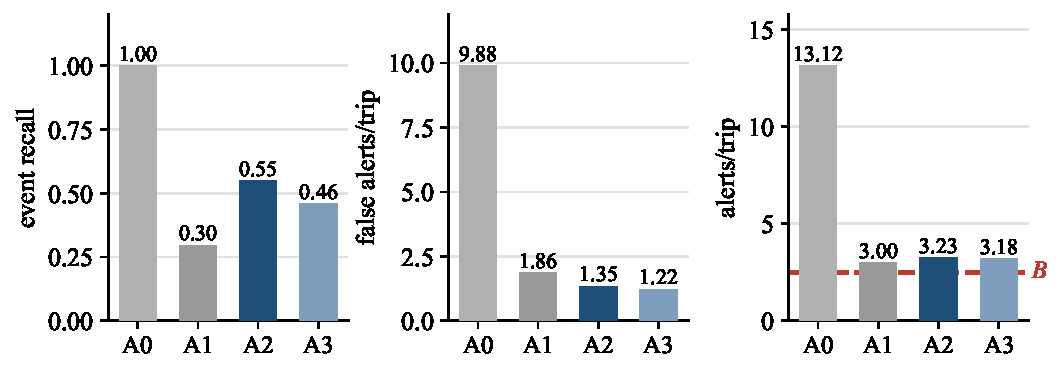
\includegraphics[width=\columnwidth]{UCC2026C_fig_aosc}
\caption{A-OSC stress regime (10 fresh seeds, frozen arms, no
re-selection). A0 produces 13.1 alerts per trip, A1 falls to 0.296
recall, and A2 retains substantially more coverage than A1 while
producing fewer alerts than A0. The dashed line marks the alert budget
$B{=}2.5$, which no arm satisfies in this regime.}
\label{fig:aosc}
\end{figure}

The four arms respond differently to the oscillatory dynamics.
A0 produces 13.1 alerts per trip, corresponding to
$5.2\times$ the declared budget, with FAR 9.9. Such a high false and
repeated alert load is consistent with conditions associated with alert
fatigue~\cite{abe2006timing,bliss2003alarm}.

A1 exhibits the opposite trade-off. Oscillation around
$\theta_{\mathrm{on}}$ repeatedly opens and closes governed events,
consuming the per-trip cap early. Its recall decreases to 0.296, with
$\ttaef=11.7$\,s.

A2 retains substantially more coverage than A1. Relative to A1, recall
increases by $+0.252$ (CI $[0.228,0.277]$), effective latency improves
by 3.5\,s (CI $[-3.88,-3.16]$), and FAR decreases by 0.51 per trip.
SAR remains zero. Maintaining fresh evidence under this regime requires
more detector executions: the force channel is activated 5.9 times per
trip, compared with 0.39 in the confirmatory holdout.

A3 again shows the effect of removing the complete evidence-aware
mechanism. Its SAR increases to 0.108
(A3 vs.\ A2 difference CI $[0.097,0.120]$), and recall is 0.089 lower
than A2.

None of the four arms satisfies the 2.5-alert budget in A-OSC. A2
produces 3.23 alerts per trip and retains only part of A0's coverage.
The stress analysis therefore does not establish robustness to arbitrary
oscillation. It shows that A2 preserves better evidence freshness and
substantially more coverage than A1 under this particular stress regime,
while still exhibiting a measurable budget violation.

\subsection{Post-hoc mechanism decomposition and baseline checks}
\label{sec:mechanism}

Three post-hoc analyses examine alternative explanations for the
confirmatory results. These analyses use no admissibility gates and do
not alter the frozen A2 configuration. Table~\ref{tab:posthoc} summarizes
their main findings.

\begin{table}[!t]
\caption{Post-hoc mechanism and baseline-robustness checks (frozen A2
configuration, no re-selection).}
\label{tab:posthoc}
\centering\scriptsize
\setlength{\tabcolsep}{4pt}
\begin{tabular}{@{}lp{4.6cm}@{}}
\toprule
Check & Main finding\\
\midrule
A4 (OSS$_t$ kept, force off) &
behavior $\approx$ A2, but SAR returns to
$0.0033$ $[0.0023,0.0044]$; 0.71 unfulfilled freshness requests/trip\\
SAR accounting threshold &
A2 SAR${}=0$ at $0.50/0.60/0.70$ (11{,}907 alerts);
A1 delivers $11.7\%$ above $0.50$\\
Re-optimized EGS (fresh seeds) &
best pure safeguard: 3.17 alerts/trip ($>B$),
FAR $0.66$ vs.\ $0.36$, SAR $0.018$ vs.\ $0$\\
\bottomrule
\end{tabular}
\end{table}

\textbf{Mechanism decomposition with A4.}
A4 separates the two mechanisms that A3 removes together, retaining
the complete OSSL evidence contract while disabling forced refresh.
The EAML can therefore
observe stale evidence and withhold an alert, but it cannot request a new
detector execution.

On the same 20 holdout seeds, A4 does not differ detectably from A2 in
recall, latency, false alerts, or alert budget, with all paired confidence
intervals containing zero. Evidence freshness differs, however. SAR
increases from zero in A2 to 0.0033 in A4
(CI $[0.0023,0.0044]$), and A4 produces 0.71 unresolved freshness
requests per trip. The same qualitative pattern is observed in A-OSC.

These results help separate the two roles. Retaining the OSSL evidence
contract is consistent with the observed admissibility, budget, latency,
and false-alert outcomes, while the force channel is associated with
eliminating the remaining stale-alert cases through fresh computation
before delivery.

\textbf{Sensitivity to the SAR accounting threshold.}
To assess whether the zero-SAR result depends on the chosen threshold of
0.60, we recomputed SAR for accounting thresholds of 0.50, 0.60, and
0.70. Across the 11{,}907 alerts delivered by A2, none has a reused ratio
above 0.50. SAR therefore remains zero under all three thresholds. In
contrast, 11.7\% of A1 alerts exceed 0.50 and 3.0\% exceed 0.60. Zero
SAR is therefore interpreted as empirical satisfaction of the
freshness-restoration invariant under the evaluated scenarios, rather
than as independent evidence of real-world safety or deployment
readiness.

\textbf{Robustness to baseline calibration.}
We also tested whether the advantage of A2 could be explained by the
pre-existing calibration of A1. The event-governed safeguard was
re-optimized over the same guard grid using the same development seeds,
and the resulting frozen design was evaluated with A2 on ten new seeds
(6001--6010).

No pure-safeguard configuration in the grid satisfies the 2.5-alert
budget on the development data. The selected configuration produces
3.17 alerts per trip on the new seeds, a 27\% budget violation, with FAR
0.66 compared with 0.36 for A2 and SAR 0.018 compared with zero.
Under the declared alert budget, the re-optimized safeguard therefore
remains inadmissible. Among the governed families evaluated in this
study, A2 remains the only admissible design.

\subsection{Runtime cost of the evidence layers}
\label{sec:cost}

After evaluating alert quality, we measure the computational overhead
introduced by the evidence-preservation and mediation layers.
Table~\ref{tab:cost} reports a microbenchmark of the three edge levels
with detector inference excluded. The benchmark processes 200{,}000
frames after 20{,}000 warm-up frames using a single-threaded pure-Python
reference implementation on a desktop-class x86-64 core.

Producing one $\osst$ requires 2.4\,$\mu$s at the median. A complete EAML
step, including the window update and RISK$\wedge$GUARD decision, requires
39\,$\mu$s, while the complete per-frame architecture with a stub
detector remains below 69\,$\mu$s at the 95th percentile. A serialized
$\osst$ occupies 402 bytes, and the full EAML window occupies at most
4.9\,KB.

At the evaluated frame rate of 9.6\,fps, corresponding to approximately
104\,ms per frame, the architecture's own processing overhead is below
0.07\% of the frame-time budget. A tenfold slowdown would still keep this
overhead below 1\,ms per frame. These measurements should not be
interpreted as embedded-hardware results. They come from unoptimized
interpreted code on x86-64; energy consumption and latency on
Raspberry-Pi- or Jetson-class platforms remain to be measured.

\begin{table}[!t]
\caption{Per-frame overhead of the evidence layers (pure Python, single
x86-64 thread, $n{=}200{,}000$ frames). The detector is a stub; costs are
the architecture's own overhead.}
\label{tab:cost}
\centering\scriptsize
\setlength{\tabcolsep}{5pt}
\begin{tabular}{@{}lrrr@{}}
\toprule
Component & p50 ($\mu$s) & p95 ($\mu$s) & Size\\
\midrule
MHEG gate decision & 0.8 & 1.4 & ---\\
OSSL $\osst$ materialization & 2.4 & 2.6 & 402\,B/$\osst$\\
EAML window step (RISK$\wedge$GUARD) & 39.4 & 59.0 &
$\leq$4.9\,KB (window)\\
Full pipeline (stub detector) & 44.8 & 68.6 & ---\\
\bottomrule
\end{tabular}
\end{table}

\section{Discussion}
\label{sec:discussion}

\textbf{Suppression evidence as an architectural requirement.}
Selective computation reduces resource use by avoiding detector
executions on frames considered redundant. The results of this study
show that this decision also affects the information available to
downstream alerting. When a frame is skipped, an alerting component may
need to know which state is being reused, how long it has been reused,
how the input has changed since the last computation, and whether fresh
inference should be requested before an alert is delivered. We refer to
this residual obligation as the \emph{evidence debt} of selective
computation.

The OSSL makes this information explicit through its per-frame evidence
contract. In the confirmatory holdout, the complete architecture produced
no alerts whose evidence windows satisfied the stale-alert criterion.
When the suppression evidence was removed in A3, stale alerts returned
and the resulting design also exceeded the alert budget. The finer A4
analysis further showed that retaining suppression evidence while
disabling forced refresh preserved most operational outcomes but no
longer produced an exact-zero SAR. Together, these results support the
role of both evidence preservation and freshness restoration in the
evaluated architecture.

This finding should be interpreted as an architectural result rather
than as evidence that the specific OSSL representation is universally
optimal; whether the same evidence fields, thresholds, and mediation
rules are appropriate in other systems requires separate evaluation.

\textbf{Why the decision levels are separated.}
The experimental arms illustrate the consequences of assigning different
responsibilities to the same mechanism. A0 directly links frame-level
detections to alerts. Under oscillating risk, repeated threshold crossings
therefore result in a high alert rate. A1 introduces event-governed
delivery, but its alert decisions still lack explicit information about
suppressed computation. Under the A-OSC regime, repeated event transitions
consume the available alert capacity early and substantially reduce
coverage.

A2 separates these responsibilities. The MHEG schedules computation,
the OSSL represents suppression, and the EAML makes the delivery
decision from accumulated evidence. The EAML can also request fresh
computation through the MHEG before an alert is delivered. The results
suggest that this separation is useful because computation scheduling,
evidence quality, and alert delivery respond to different operational
constraints.

\textbf{Trade-off introduced by freshness restoration.}
The zero-SAR result does not come without additional computation.
Freshness restoration required 0.39 forced computations per trip in the
confirmatory holdout and 5.9 per trip in the oscillating-risk analysis.
The increased use of the force channel under stress is consistent with
its intended role: more uncertain or reuse-dominated evidence results in
more requests for fresh inference.

The comparison with A0 also shows why raw latency alone cannot
characterize alert quality: its lower latency comes with 3.49 alerts
per trip (39\% over budget) and substantially higher FAR. Among the
governed designs, A2 and A1
operate at similar effective latency, while A2 reduces false alerts,
redundant alerts, and stale alerts and remains within the alert budget.
The relevant trade-off in this study is therefore between responsiveness,
alert burden, and evidence quality rather than latency alone.

\textbf{Role of explicit admissibility criteria.}
The amendment trail shows that the acceptance criteria were capable of
rejecting candidate designs: two specifications were rejected with
empty admissible sets before the final protocol adopted non-inferiority
requirements together with explicit quality and budget constraints.
These earlier empty sets are retained because they clarify how the
final hypothesis was formed and demonstrate that acceptance was not
guaranteed by the evaluation procedure.

\textbf{Scope and transferability.}
The architecture was evaluated for vehicular risk communication, but the
underlying problem is not specific to driving. Other edge systems may
also suppress expensive computation while later making decisions from
reused inference. In such systems, preserving information about skipped
computation may help downstream components distinguish fresh evidence
from reused evidence.

Different applications would require their own detectors,
evidence-quality definitions, budgets, thresholds, and validation
procedures. The transferable claim
is therefore limited to the architectural principle that suppression and
downstream decision making should not be treated as independent when the
latter depends on the freshness of the former.

\section{Threats to Validity}
\label{sec:threats}

\textbf{Construct validity.}
The evaluation measures properties of risk communication rather than
post-alert driving outcomes. Event recall, effective latency, FAR,
redundant alerts, and SAR characterize whether and how alerts are
delivered, but they do not measure whether the driver subsequently
responds correctly or whether an unsafe event is prevented. The synthetic
driver-response model is used only as part of the experimental dynamics
and should not be interpreted as a validated behavioral model.

The alert budget, the non-inferiority margins, and the $0.60$ reuse
threshold are operational definitions used by this study rather than
universal human-factors constants. Their provenance is reported
explicitly in Sections~\ref{sec:arch} and~\ref{sec:protocol}.

\textbf{Internal validity.}
All arms use the same episode generator, observation model, MHEG
configuration, and pre-drawn exogenous realizations. Common random
numbers are verified programmatically, and inference is based on paired
persona$\times$seed differences. Development and holdout seeds are
disjoint, and the confirmatory holdout was executed once after the
configuration and final admissibility specification were frozen.

The freezing procedure is programmatic rather than externally
preregistered. In addition, the 1.0\,s latency non-inferiority margin was
chosen after development-data inspection. The methodological protection
is instead the
separation between development and the untouched holdout, together with
the preserved amendment trail.

A1 is a previously frozen event-governed baseline and was not originally
optimized for the current experiment. This could create a calibration
advantage for A2. The post-hoc baseline check addresses this concern by
re-optimizing the safeguard using the same development seeds and testing
the resulting configuration on fresh seeds. No evaluated pure-safeguard
configuration satisfies the declared alert budget, although this result
is limited to the explored parameter grid and generator.

\textbf{External validity.}
All behavioral episodes and driver personas are synthetic. Feature and
risk calibration draw on naturalistic-driving statistics, but the
observation and response processes are declared models rather than
models learned from naturalistic trajectories. The reported results
therefore characterize the evaluated synthetic environment and should
not be interpreted as estimates of real-world driver behavior.

The personas encode risk, responsiveness, and fatigue parameters for
experimental variation only and support no demographic or population
claims. Similarly, A-OSC is a deliberately constructed stress regime
designed to exercise interactions between suppression and alert
governance. It represents one out-of-nominal condition rather than a
realistic distribution-shift model.

\textbf{Implementation validity.}
The computational-cost measurements were obtained from a single-threaded
pure-Python reference implementation on a desktop-class x86-64 processor.
They isolate the overhead of the proposed architecture and exclude the
cost of the detector itself. Although the measured overhead is small
relative to the evaluated frame period, these results are not equivalent
to measurements on automotive or embedded hardware. Runtime latency,
energy consumption, memory behavior, and thermal constraints on
Raspberry-Pi-, Jetson-, or automotive-grade platforms remain to be
measured.

\section{Conclusion}
\label{sec:conclusion}

We presented a cognitive edge architecture that separates selective
computation, suppression-evidence preservation, episodic alert delivery,
and slower configuration adaptation. Its central mechanism is a
per-frame evidence contract that makes skipped computation observable to
the alerting layer, together with a single mediated origin for driver
alerts.

Under the frozen 20-seed confirmatory holdout, the complete architecture
satisfied all pre-declared admissibility gates relative to the
event-governed baseline. Event recall increased by 0.021 at effective
latency parity, false alerts per trip decreased by 62\%, and SAR decreased
from 0.030 to zero. Removing the suppression-evidence mechanism made the
resulting design inadmissible and reintroduced stale alerts.

The oscillating-risk analysis showed a different operating regime. A0
produced 13.1 alerts per trip, A1 recall decreased to 0.296, and A2
retained substantially more coverage than A1 while empirically
satisfying the zero-stale-alert invariant under the evaluated
accounting thresholds. However, A2 also exceeded the alert budget in this regime.
These results therefore indicate improved evidence quality and alert
behavior under the evaluated stress condition rather than immunity to
out-of-nominal dynamics.

Within the synthetic environment considered here, the results support a
specific architectural principle: when an edge system suppresses
computation, downstream communication decisions should have explicit
access to information about the resulting evidence freshness. Future
work will evaluate this principle using naturalistic driving data,
measure its computational and energy cost on embedded hardware, and test
the evidence contract in a second application domain.

\section*{Artifact Availability}

The artifact contains the episode generator, behavioral recipes,
synthetic personas, implementations of the evaluated arms, all three
protocol specifications, the two empty-set development outcomes, the
frozen confirmatory configuration and holdout outputs, the A-OSC stress
analysis, mechanism-decomposition and baseline-robustness results, the
runtime microbenchmark, and a SHA-256 integrity manifest. An anonymized
artifact containing the code, frozen configurations, seeds, raw
outputs, table-generation scripts, and SHA-256 manifest is provided as
supplementary material. The archival repository and DOI will be
disclosed in the camera-ready version.

\section*{Acknowledgment of Generative AI Use}

Anthropic Claude (Fable 5) assisted with language editing throughout
Sections I--VIII and with the development and review of the
experimental code. The research questions, architecture, experimental protocol, implementation decisions, result validation, scientific interpretation, and conclusions remained with the authors. All AI-assisted outputs were reviewed by the authors, who retain final responsibility for the manuscript.

\begin{thebibliography}{23}
\bibitem{shi2016edge} W.~Shi, J.~Cao, Q.~Zhang, Y.~Li, and L.~Xu, ``Edge
computing: Vision and challenges,'' \emph{IEEE Internet Things J.},
vol.~3, no.~5, pp.~637--646, 2016.
\bibitem{liu2019autonomous} S.~Liu \emph{et al.}, ``Edge computing for
autonomous driving: Opportunities and challenges,'' \emph{Proc. IEEE},
vol.~107, no.~8, pp.~1697--1716, 2019.
\bibitem{campos2018skiprnn} V.~Campos, B.~Jou, X.~Gir\'o-i-Nieto,
J.~Torres, and S.-F. Chang, ``Skip RNN: Learning to skip state updates in
recurrent neural networks,'' in \emph{Proc. ICLR}, 2018.
\bibitem{graves2016act} A.~Graves, ``Adaptive computation time for
recurrent neural networks,'' in \emph{Adv. Neural Inf. Process. Syst.
(NeurIPS)}, 2016.
\bibitem{wu2019adaframe} Z.~Wu, C.~Xiong, C.-Y. Ma, R.~Socher, and
L.~S. Davis, ``AdaFrame: Adaptive frame selection for fast video
recognition,'' in \emph{Proc. IEEE/CVF CVPR}, 2019, pp.~1278--1287.
\bibitem{wu2019liteeval} Z.~Wu, C.~Xiong, Y.-G. Jiang, and L.~S. Davis,
``LiteEval: A coarse-to-fine framework for resource efficient video
recognition,'' in \emph{Adv. Neural Inf. Process. Syst. (NeurIPS)}, 2019.
\bibitem{xu2021oad} M.~Xu, Y.~Xiong, H.~Chen, X.~Li, W.~Xia, Z.~Tu, and
S.~Soatto, ``Long short-term transformer for online action detection,''
in \emph{Adv. Neural Inf. Process. Syst. (NeurIPS)}, 2021,
pp.~22\,610--22\,622.
\bibitem{sajid2021}
F.~Sajid, A.~R. Javed, A.~Basharat, N.~Kryvinska, A.~Afzal,
and M.~Rizwan, ``An efficient deep learning framework for distracted
driver detection,'' \emph{IEEE Access}, vol.~9, 2021,
doi: 10.1109/ACCESS.2021.3138137.
\bibitem{fresta2025}
M.~Fresta, F.~Bellotti, I.~Bochenko, L.~Lazzaroni, G.~Merlhiot,
F.~Tango, and R.~Berta,
``Deep learning-based real-time driver cognitive distraction detection,''
\emph{IEEE Access}, vol.~13, pp.~26\,589--26\,607, 2025,
doi: 10.1109/ACCESS.2025.3539392.
\bibitem{kephart2003} J.~O. Kephart and D.~M. Chess, ``The vision of
autonomic computing,'' \emph{Computer}, vol.~36, no.~1, pp.~41--50, 2003.
\bibitem{weyns2020} D.~Weyns, \emph{An Introduction to Self-Adaptive
Systems: A Contemporary Software Engineering Perspective}. Wiley--IEEE
Press, 2020.
\bibitem{seto1998simplex} D.~Seto, B.~Krogh, L.~Sha, and A.~Chutinan,
``The Simplex architecture for safe online control system upgrades,'' in
\emph{Proc. ACC}, vol.~6, 1998, pp.~3504--3508.
\bibitem{alshiekh2018shield} M.~Alshiekh, R.~Bloem, R.~Ehlers,
B.~K\"onighofer, S.~Niekum, and U.~Topcu, ``Safe reinforcement learning
via shielding,'' in \emph{Proc. AAAI}, 2018, pp.~2669--2678.
\bibitem{abe2006timing} G.~Abe and J.~Richardson, ``Alarm timing, trust
and driver expectation for forward collision warning systems,''
\emph{Appl. Ergon.}, vol.~37, no.~5, pp.~577--586, 2006.
\bibitem{bliss2003alarm} J.~P. Bliss and S.~A. Acton, ``Alarm mistrust in
automobiles: How collision alarm reliability affects driving,''
\emph{Appl. Ergon.}, vol.~34, no.~6, pp.~499--509, 2003.
\bibitem{dingus2016shrp2} T.~A. Dingus, F.~Guo, S.~Lee, J.~F. Antin,
M.~Perez, M.~Buchanan-King, and J.~Hankey, ``Driver crash risk factors
and prevalence evaluation using naturalistic driving data,'' \emph{Proc.
Natl. Acad. Sci. U.S.A.}, vol.~113, no.~10, pp.~2636--2641, 2016.
\bibitem{law2015} A.~M. Law, \emph{Simulation Modeling and Analysis},
5th ed. McGraw-Hill, 2015.
\bibitem{yates2021aoi} R.~D. Yates, Y.~Sun, D.~R. Brown~III, S.~K. Kaul,
E.~Modiano, and S.~Ulukus, ``Age of information: An introduction and
survey,'' \emph{IEEE J. Sel. Areas Commun.}, vol.~39, no.~5,
pp.~1183--1210, 2021.
\bibitem{shisher2022freshness} M.~K.~C. Shisher and Y.~Sun, ``How does
data freshness affect real-time supervised learning?'' in \emph{Proc.
ACM MobiHoc}, 2022.
\bibitem{gokarn2023mosaic} I.~Gokarn, H.~Sabbella, Y.~Hu,
T.~Abdelzaher, and A.~Misra, ``MOSAIC: Spatially-multiplexed edge AI
optimization over multiple concurrent video sensing streams,'' in
\emph{Proc. ACM MMSys}, 2023.
\bibitem{zhu2026paoi}
J.~Zhu and J.~Gong,
``Multi-source peak age of information optimization in mobile edge
computing systems,'' \emph{IEEE/ACM Trans. Netw.}, 2025.
\bibitem{bui2024timely} V.-P. Bui, S.~R. Pandey, P.~M. de~Sant~Ana,
B.~Soret, and P.~Popovski, ``Timely communication from sensors for
wireless networked control in cloud-based digital twins,'' arXiv
preprint arXiv:2408.10241, 2024.
\bibitem{hochreiter1997} S.~Hochreiter and J.~Schmidhuber, ``Long
short-term memory,'' \emph{Neural Comput.}, vol.~9, pp.~1735--1780,
1997.
\end{thebibliography}

\end{document}
